\documentclass[12pt]{article}
\usepackage{amsmath, amsthm, amssymb}
\usepackage{hyperref}
\usepackage{verbatim}
\usepackage{fullpage}

\pagestyle{plain}

\usepackage{tkz-graph}
\usetikzlibrary{arrows}
\usetikzlibrary{shapes}
\usepackage[position=bottom]{subfig}

\usepackage{longtable}
\usepackage{array}

\usepackage{sectsty}
\allsectionsfont{\sffamily}

\setcounter{secnumdepth}{5}
\setcounter{tocdepth}{5}

\makeatletter
\newtheorem*{rep@theorem}{\rep@title}
\newcommand{\newreptheorem}[2]{
\newenvironment{rep#1}[1]{
 \def\rep@title{#2 \ref{##1}}
 \begin{rep@theorem}}
 {\end{rep@theorem}}}
\makeatother

\theoremstyle{plain}
\newtheorem{thm}{Theorem}[section]
\newreptheorem{thm}{Theorem}
\newtheorem{prop}[thm]{Proposition}
\newreptheorem{prop}{Proposition}
\newtheorem{lem}[thm]{Lemma}
\newreptheorem{lem}{Lemma}
\newtheorem{conjecture}[thm]{Conjecture}
\newreptheorem{conjecture}{Conjecture}
\newtheorem{cor}[thm]{Corollary}
\newreptheorem{cor}{Corollary}
\newtheorem{prob}[thm]{Problem}
\newtheorem{observation}{Observation}
\newtheorem*{mainconj}{Main Conjecture}
\newtheorem*{mainthm}{Main Theorem}

\theoremstyle{definition}
\newtheorem{defn}{Definition}
\theoremstyle{remark}
\newtheorem*{remark}{Remark}
\newtheorem*{problem}{Problem}
\newtheorem{example}{Example}
\newtheorem*{question}{Question}


\newcommand{\fancy}[1]{\mathcal{#1}}
\newcommand{\C}[1]{\fancy{C}_{#1}}
\newcommand{\IN}{\mathbb{N}}
\newcommand{\IR}{\mathbb{R}}
\newcommand{\G}{\fancy{G}}
\newcommand{\CC}{\fancy{C}}
\newcommand{\D}{\fancy{D}}

\newcommand{\inj}{\hookrightarrow}
\newcommand{\surj}{\twoheadrightarrow}

\newcommand{\set}[1]{\left\{ #1 \right\}}
\newcommand{\setb}[3]{\left\{ #1 \in #2 \mid #3 \right\}}
\newcommand{\setbs}[2]{\left\{ #1 \mid #2 \right\}}
\newcommand{\card}[1]{\left|#1\right|}
\newcommand{\size}[1]{\left\Vert#1\right\Vert}
\newcommand{\ceil}[1]{\left\lceil#1\right\rceil}
\newcommand{\floor}[1]{\left\lfloor#1\right\rfloor}
\newcommand{\func}[3]{#1\colon #2 \rightarrow #3}
\newcommand{\funcinj}[3]{#1\colon #2 \inj #3}
\newcommand{\funcsurj}[3]{#1\colon #2 \surj #3}
\newcommand{\irange}[1]{\left[#1\right]}
\newcommand{\join}[2]{#1 \mbox{\hspace{2 pt}$\ast$\hspace{2 pt}} #2}
\newcommand{\djunion}[2]{#1 \mbox{\hspace{2 pt}$+$\hspace{2 pt}} #2}
\newcommand{\parens}[1]{\left( #1 \right)}
\newcommand{\brackets}[1]{\left[ #1 \right]}
\newcommand{\nint}[1]{\widetilde{N}\left(#1\right)}
\newcommand{\DefinedAs}{\mathrel{\mathop:}=}
\newcommand{\pot}{\operatorname{pot}}

\def\adj{\leftrightarrow}
\def\nonadj{\not\!\leftrightarrow}

\def\D{\fancy{D}}
\def\C{\fancy{C}}
\def\Q{\fancy{Q}}
\def\Z{\fancy{Z}}
\def\K{\fancy{K}}

\newcommand{\case}[2]{{\bf Case #1.}~{\it #2}~~}
\newcommand{\claim}[2]{{\bf Claim #1.}~{\it #2}~~}

\newcommand{\wild}{\raisebox{0.75\depth}{$\bigstar$}}


\begin{document}
\title{fixable proofs}
\maketitle

\section{Proofs}
\begin{figure}
	\centering
	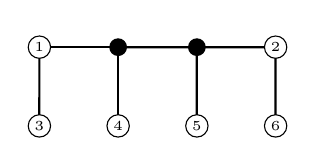
\begin{tikzpicture}[scale = 10]
	\tikzstyle{VertexStyle} = []
	\tikzstyle{EdgeStyle} = []
	\tikzstyle{labeledStyle}=[shape = circle, minimum size = 6pt, inner sep = 1.2pt, draw]
	\tikzstyle{unlabeledStyle}=[shape = circle, minimum size = 6pt, inner sep = 1.2pt, draw, fill]
	\Vertex[style = labeledStyle, x = 0.55, y = 0.75, L = \tiny {$1$}]{v0}
	\Vertex[style = unlabeledStyle, x = 0.65, y = 0.75, L = \tiny {}]{v1}
	\Vertex[style = unlabeledStyle, x = 0.75, y = 0.75, L = \tiny {}]{v2}
	\Vertex[style = labeledStyle, x = 0.85, y = 0.75, L = \tiny {$2$}]{v3}
	\Vertex[style = labeledStyle, x = 0.55, y = 0.65, L = \tiny {$3$}]{v4}
	\Vertex[style = labeledStyle, x = 0.65, y = 0.65, L = \tiny {$4$}]{v5}
	\Vertex[style = labeledStyle, x = 0.75, y = 0.65, L = \tiny {$5$}]{v6}
	\Vertex[style = labeledStyle, x = 0.85, y = 0.65, L = \tiny {$6$}]{v7}
	\Edge[label = \tiny {}, labelstyle={auto=right, fill=none}](v1)(v0)
	\Edge[label = \tiny {}, labelstyle={auto=right, fill=none}](v1)(v2)
	\Edge[label = \tiny {}, labelstyle={auto=right, fill=none}](v1)(v5)
	\Edge[label = \tiny {}, labelstyle={auto=right, fill=none}](v3)(v2)
	\Edge[label = \tiny {}, labelstyle={auto=right, fill=none}](v3)(v7)
	\Edge[label = \tiny {}, labelstyle={auto=right, fill=none}](v4)(v0)
	\Edge[label = \tiny {}, labelstyle={auto=right, fill=none}](v6)(v2)
	\end{tikzpicture}
	
	\caption{Solid vertices have lists of size 3 and the labeled vertices have lists of size 2.}\label{fig:e03d91ed-07f8-410a-b17e-6e7679e7e6e0}
\end{figure}
\begin{lem}
	The graph in Figure \ref{fig:e03d91ed-07f8-410a-b17e-6e7679e7e6e0} is reducible.
\end{lem}
\begin{proof}Let $X = \{0,1\}$, $Y = \{0,2\}$ and $Z = \{1,2\}$. Then with the vertex ordering in Figure \ref{fig:e03d91ed-07f8-410a-b17e-6e7679e7e6e0}, a string such as YXYZZY, 
	represents a possible list assignment on $V(H)$ arising from a $3$-edge-coloring of $G-E(H)$.
	By an $X$-Kempe change, we mean flipping colors $0$ and $1$ on a two-colored path in $G-E(H)$.  We call such a path an $X$-path. 
	Any endpoint of an $X$-path in $H$ must end at a $Y$ or $Z$ vertex.  The meanings of $Y$-Kempe change, $Z$-Kempe change, $Y$-path and $Z$-path are analogous.
	Note that if there are an odd number of $Y$'s and $Z$'s, then at least one $X$-path has only one endpoint in $H$.
	We use shorthand notation like $\K_{X, 2}(YXYZZY,5,6) \Rightarrow YYYXZY,ZZZXYZ$ (Case 1).
	This means the $X$-Kempe change on YXYZZY starting at the second vertex and ending at the fifth and sixth result in boards YYYXZY and ZZZXYZ respectively and these are handled by Case 1.
	The $\infty$ symbol means starting (or ending) outside $H$.
	
	We need to handle all boards up to permutations of $\{X,Y,Z\}$, so it will suffice to handle all boards of the form $\wild \wild \wild \wild YZ$, $\wild \wild \wild YZZ$, $\wild \wild YZZZ$, $\wild YZZZZ$, $YZZZZZ$ or $ZZZZZZ$.
	
	
	\bigskip
	\case{1}{$B$ is one of $\wild Z\wild \wild YZ$, $\wild Y\wild YZZ$, $\wild X\wild YZZ$, $\wild \wild ZYYZ$, $\wild \wild XYYZ$, $Y\wild Y\wild YZ$, $\wild ZYZZZ$, $X\wild ZZYZ$, $X\wild XZYZ$, $Y\wild YZZZ$, $Y\wild ZZYZ$, $Y\wild XXYZ$, $Z\wild ZXYZ$, $Z\wild XXYZ$, $XYZZZZ$, $XZYYZZ$, $XZXYZZ$, $YYZZZZ$, $ZZZZZZ$, $ZZZYZZ$ or $ZZYYZZ$.}
	
	\bigskip
	
	In all these cases, $H$ is immediately colorable from the lists.
	
	
	\bigskip
	\case{2}{$B$ is one of $XYY\wild YZ$, $ZY\wild ZYZ$, $XXYZYZ$, $XXYXYZ$, $XYYZZZ$, $XZZYZZ$, $YYXZYZ$, $YZYYZZ$, $YZZYZZ$, $YZZZZZ$, $ZXYZYZ$, $ZXYYYZ$, $ZXZZYZ$, $ZXYZZZ$, $ZYYYYZ$, $ZYYZZZ$ or $ZYZZZZ$.}
	
	\bigskip
	
	$\K_{Y,3}(YZZZZZ,\infty,4, 5, 6)\Rightarrow $$XZYZZZ$, $XZYYZZ$, $XZYZYZ$, $XYZYYZ$(Case 1).
	
	$\K_{Y,5}(YZZZZZ,\infty,4, 6)\Rightarrow $$XZZZYZ$, $XZZYYZ$, $XYYYZZ$(Case 1).
	
	$\K_{Y,2}(YZZZZZ,\infty)\Rightarrow $$XYZZZZ$(Case 1).
	
	
	
	$(2 1 4 3 6 5)\Rightarrow ZYZZZZ$
	
	
	
	$\K_{X,3}(ZYYZZZ,2, 4, 6)\Rightarrow $$ZZZZZZ$, $ZYZYZZ$, $YZYYYZ$(Case 1).
	
	$\K_{X,4}(ZYYZZZ,2, 6)\Rightarrow $$ZZYYZZ$, $YZZZYZ$(Case 1).
	
	$\K_{X,2}(ZYYZZZ,6)\Rightarrow $$YYZYYZ$(Case 1).
	
	
	
	$(1 2 5 4 3 6)\Rightarrow ZYZZYZ$
	
	$(2 1 4 3 6 5)\Rightarrow YZZYZZ$
	
	$(2 1 6 3 4 5)\Rightarrow ZYYYYZ$
	
	
	
	$\K_{X,6}(ZXYZZZ,\infty,1, 3, 4, 5)\Rightarrow $$YXZYYZ$, $ZXZYYZ$, $YXYYYZ$, $YXZZYZ$, $YXZYZZ$(Case 1).
	
	$\K_{X,4}(ZXYZZZ,\infty,3)\Rightarrow $$ZXYYZZ$, $ZXZYZZ$(Case 1).
	
	$\K_{X,1}(ZXYZZZ,\infty)\Rightarrow $$YXYZZZ$(Case 1).
	
	
	
	$(1 2 5 4 3 6)\Rightarrow ZXZZYZ$
	
	$(2 1 4 5 6 3)\Rightarrow XZZYZZ$
	
	$(2 1 6 5 4 3)\Rightarrow XYYYYZ$
	
	
	
	$\K_{X,3}(XYYZZZ,\infty,4, 6)\Rightarrow $$XYZZZZ$, $XYZYZZ$, $XZYYYZ$(Case 1).
	
	$\K_{X,4}(XYYZZZ,\infty,6)\Rightarrow $$XYYYZZ$, $XZZZYZ$(Case 1).
	
	$\K_{X,2}(XYYZZZ,\infty)\Rightarrow $$XZYZZZ$(Case 1).
	
	$\K_{X,6}(XYYZZZ,\infty)\Rightarrow $$XZZYYZ$(Case 1).
	
	
	
	$(2 1 6 3 4 5)\Rightarrow ZXYYYZ$
	
	
	
	$\K_{X,4}(YZYYZZ,2, 5, 6)\Rightarrow $$YYYZZZ$, $YZYZYZ$, $ZYZYYZ$(Case 1).
	
	$\K_{X,2}(YZYYZZ,1, 3, 5, 6)\Rightarrow $$ZYYYZZ$, $YYZYZZ$, $YYYYYZ$, $ZZZZYZ$(Case 1).
	
	$\K_{X,3}(YZYYZZ,5)\Rightarrow $$YZZYYZ$(Case 1).
	
	
	
	$(1 2 6 4 5 3)\Rightarrow ZYYZYZ$
	
	
	
	$\K_{X,6}(ZXYZYZ,\infty,1, 3, 4, 5)\Rightarrow $$YXZYZZ$, $ZXZYZZ$, $YXYYZZ$, $XYZZZZ$, $YXZYYZ$(Case 1).
	
	$\K_{X,1}(ZXYZYZ,\infty)\Rightarrow $$YXYZYZ$(Case 1).
	
	$\K_{X,4}(ZXYZYZ,3, 5)\Rightarrow $$ZXZYYZ$, $ZXYYZZ$(Case 1).
	
	
	
	$(2 1 4 5 6 3)\Rightarrow XYYZYZ$
	
	
	
	$\K_{X,4}(ZYXZYZ,\infty,2, 5, 6)\Rightarrow $$ZYXYYZ$, $ZZXYYZ$, $ZYXYZZ$, $XZYZZZ$(Case 1).
	
	$\K_{X,2}(ZYXZYZ,\infty,5, 6)\Rightarrow $$ZZXZYZ$, $ZZYZZZ$, $YYXYZZ$(Case 1).
	
	$\K_{X,5}(ZYXZYZ,6)\Rightarrow $$YZXYYZ$(Case 1).
	
	
	
	$(1 4 3 2 6 5)\Rightarrow YYXZYZ$
	
	$(2 1 6 5 4 3)\Rightarrow XYYXYZ$
	
	$(2 5 6 1 3 4)\Rightarrow XXYXYZ$
	
	
	
	$\K_{X,4}(XXYZYZ,5, 6)\Rightarrow $$XXYYZZ$, $YYZZZZ$(Case 1).
	
	$\K_{X,5}(XXYZYZ,6)\Rightarrow $$XXZYYZ$(Case 1).
	
	
	
	\bigskip
	\case{3}{$B$ is one of $XYZXYZ$, $XXXXYZ$, $XXZXYZ$, $XYXXYZ$, $XXYYYZ$, $XXYZZZ$, $YXXZYZ$, $YYZXYZ$, $YZXYZZ$, $ZXYXYZ$, $ZZXYZZ$, $ZXXZYZ$ or $ZYYXYZ$.}
	
	\bigskip
	
	$\K_{Z,\infty}(XXYZZZ,1, 2, 3)\Rightarrow $$YXYZZZ$, $XYYZZZ$, $YYYZZZ$( Case 1 and 2).
	
	
	
	$(1 2 6 3 4 5)\Rightarrow XXYYYZ$
	
	$(1 4 3 2 5 6)\Rightarrow YZXYZZ$
	
	$(1 6 4 2 3 5)\Rightarrow ZYYXYZ$
	
	$(2 3 5 1 4 6)\Rightarrow ZXXZYZ$
	
	$(2 5 6 1 3 4)\Rightarrow XYXXYZ$
	
	$(3 6 4 1 2 5)\Rightarrow YYZXYZ$
	
	$(3 6 5 1 2 4)\Rightarrow XXZXYZ$
	
	
	
	$\K_{X,4}(ZZXYZZ,\infty,2, 5, 6)\Rightarrow $$ZZYZZZ$, $ZXYZZZ$, $ZZXZYZ$, $YYXYYZ$(Case 1 and 2).
	
	$\K_{X,2}(ZZXYZZ,\infty)\Rightarrow $$ZYXYZZ$(Case 1).
	
	$\K_{X,5}(ZZXYZZ,\infty)\Rightarrow $$ZZXYYZ$(Case 1).
	
	$\K_{X,6}(ZZXYZZ,\infty)\Rightarrow $$YYXZYZ$(Case 2).
	
	
	
	$(2 1 6 5 3 4)\Rightarrow XXXXYZ$
	
	
	
	$\K_{X,4}(YXXZYZ,5, 6)\Rightarrow $$YXXYZZ$, $ZYYZZZ$(Case 1 and 2).
	
	$\K_{X,5}(YXXZYZ,6)\Rightarrow $$ZXXYYZ$(Case 1).
	
	
	
	$(1 2 5 3 4 6)\Rightarrow XYZXYZ$
	
	$(1 3 5 2 6 4)\Rightarrow ZXYXYZ$
	
	
	
	
	
	\bigskip
	\case{4}{$B$ is one of $YXZXYZ$.}
	
	\bigskip
	
	$\K_{X,3}(YXZXYZ,5, 6)\Rightarrow $$XYXYZZ$, $ZYZYZZ$(Case 1).
	
	$\K_{X,5}(YXZXYZ,6)\Rightarrow $$ZXYXYZ$(Case 3).
	
	
\end{proof}


\end{document}

